%%%%%%%%%%%%%%%%%%%%%%%%%%%%
% Two Sword Lengths Apart: Supplementary Material
% 25 March 2014
%%%%%%%%%%%%%%%%%%%%%%%%%%%%

% !Rnw weave = knitr

\documentclass[a4paper]{article}\usepackage[]{graphicx}\usepackage[]{color}
%% maxwidth is the original width if it is less than linewidth
%% otherwise use linewidth (to make sure the graphics do not exceed the margin)
\makeatletter
\def\maxwidth{ %
  \ifdim\Gin@nat@width>\linewidth
    \linewidth
  \else
    \Gin@nat@width
  \fi
}
\makeatother

\definecolor{fgcolor}{rgb}{0.345, 0.345, 0.345}
\newcommand{\hlnum}[1]{\textcolor[rgb]{0.686,0.059,0.569}{#1}}%
\newcommand{\hlstr}[1]{\textcolor[rgb]{0.192,0.494,0.8}{#1}}%
\newcommand{\hlcom}[1]{\textcolor[rgb]{0.678,0.584,0.686}{\textit{#1}}}%
\newcommand{\hlopt}[1]{\textcolor[rgb]{0,0,0}{#1}}%
\newcommand{\hlstd}[1]{\textcolor[rgb]{0.345,0.345,0.345}{#1}}%
\newcommand{\hlkwa}[1]{\textcolor[rgb]{0.161,0.373,0.58}{\textbf{#1}}}%
\newcommand{\hlkwb}[1]{\textcolor[rgb]{0.69,0.353,0.396}{#1}}%
\newcommand{\hlkwc}[1]{\textcolor[rgb]{0.333,0.667,0.333}{#1}}%
\newcommand{\hlkwd}[1]{\textcolor[rgb]{0.737,0.353,0.396}{\textbf{#1}}}%

\usepackage{framed}
\makeatletter
\newenvironment{kframe}{%
 \def\at@end@of@kframe{}%
 \ifinner\ifhmode%
  \def\at@end@of@kframe{\end{minipage}}%
  \begin{minipage}{\columnwidth}%
 \fi\fi%
 \def\FrameCommand##1{\hskip\@totalleftmargin \hskip-\fboxsep
 \colorbox{shadecolor}{##1}\hskip-\fboxsep
     % There is no \\@totalrightmargin, so:
     \hskip-\linewidth \hskip-\@totalleftmargin \hskip\columnwidth}%
 \MakeFramed {\advance\hsize-\width
   \@totalleftmargin\z@ \linewidth\hsize
   \@setminipage}}%
 {\par\unskip\endMakeFramed%
 \at@end@of@kframe}
\makeatother

\definecolor{shadecolor}{rgb}{.97, .97, .97}
\definecolor{messagecolor}{rgb}{0, 0, 0}
\definecolor{warningcolor}{rgb}{1, 0, 1}
\definecolor{errorcolor}{rgb}{1, 0, 0}
\newenvironment{knitrout}{}{} % an empty environment to be redefined in TeX

\usepackage{alltt}
\usepackage{fullpage}
\usepackage{lscape}
\usepackage[authoryear]{natbib}
\usepackage{setspace}
    \doublespacing
\usepackage{hyperref}
\hypersetup{
    colorlinks,
    citecolor=black,
    filecolor=black,
    linkcolor=cyan,
    urlcolor=cyan
}
\usepackage{booktabs}
\usepackage{dcolumn}
\usepackage{url}
\usepackage{tikz}
\usepackage{todonotes}
\usepackage{verbatim}
\usepackage{endnotes}
\usepackage{graphicx}
\usepackage{float}

\usepackage[margins]{trackchanges}

\usepackage{footmisc}
\setlength{\footnotesep}{\baselineskip}
\renewcommand{\footnotelayout}{\doublespacing\normalsize}

\renewcommand*\thetable{\Roman{table}}
\setlength{\belowcaptionskip}{0.5cm}

%%%%%%% Title Page %%%%%%%%%%%%%%%%%%%%%%%%%%%%%%%%%%%%%%%%%%%%
\title{Supplementary Material: Two Sword Lengths Apart: Credible Commitment Problems and Physical Violence in Democratic National Legislatures}
\IfFileExists{upquote.sty}{\usepackage{upquote}}{}
\begin{document}

\maketitle



%%%%%%%%%%%%%%%% Run Analyses %%%%%%%%%%%%%%%%%%%%%%%%



\section*{Examining Possible Measurement Error: Trends in Violence and Democracy}

\todo[inline]{Section added.}

As noted in the main text, data on incidents was primarily gathered using multiple key word searches of the Google News Archive, Google Search, and Youtube over a number of years. This method could have significant measurement error. The electronic availability of news and videos on legislative violence, as with material on almost all other phenomenon, could be positively correlated with time. I.e. more information is available for incidents in more recent periods.

There are more incidents in later periods of the data set than earlier periods. For example, there were only 8 incidents observed in the 1980s, but 65 in the sample's last ten years (2002-2012). However, there are good reasons to believe that this distribution of incidents in time is not simply the result of measurement error.

Primarily, there are many more countries with multi-party elected national legislatures--the criteria for inclusion--that could have violence later in the sample. The top panel of Figure \ref{elect_vs_violence} shows the number of countries in the sample with elected multi-party national legislatures. In 1981 there were only 65 countries. Between 1990 and 1995 a dramatic increase occurred such that by 1995 135 countries had multi-party elected legislatures. At the end of the sample period, almost double the original number 149 countries have multi-party elected national legislatures. In the bottom panel of Figure \ref{elect_vs_violence} we can see that the average observed number of violent incidents roughly follows the pattern of democratization. There is a noticeable increase in the average number of violent incidents from the mid-1990s. Furthermore, as the empirical evidence in this article has demonstrated newer democracies are more likely to have legislative violence. As such, we should expect to see more violence in the more recent period when there are many new democracies.

Measurement error caused by the electronic availability of information be an issue. Nonetheless, the increasing prevalence of young multi-party elected national legislatures is likely an important cause of there being more observed incidents of violence later in the sample.

\begin{figure}

    \begin{center}
\begin{knitrout}
\definecolor{shadecolor}{rgb}{0.969, 0.969, 0.969}\color{fgcolor}
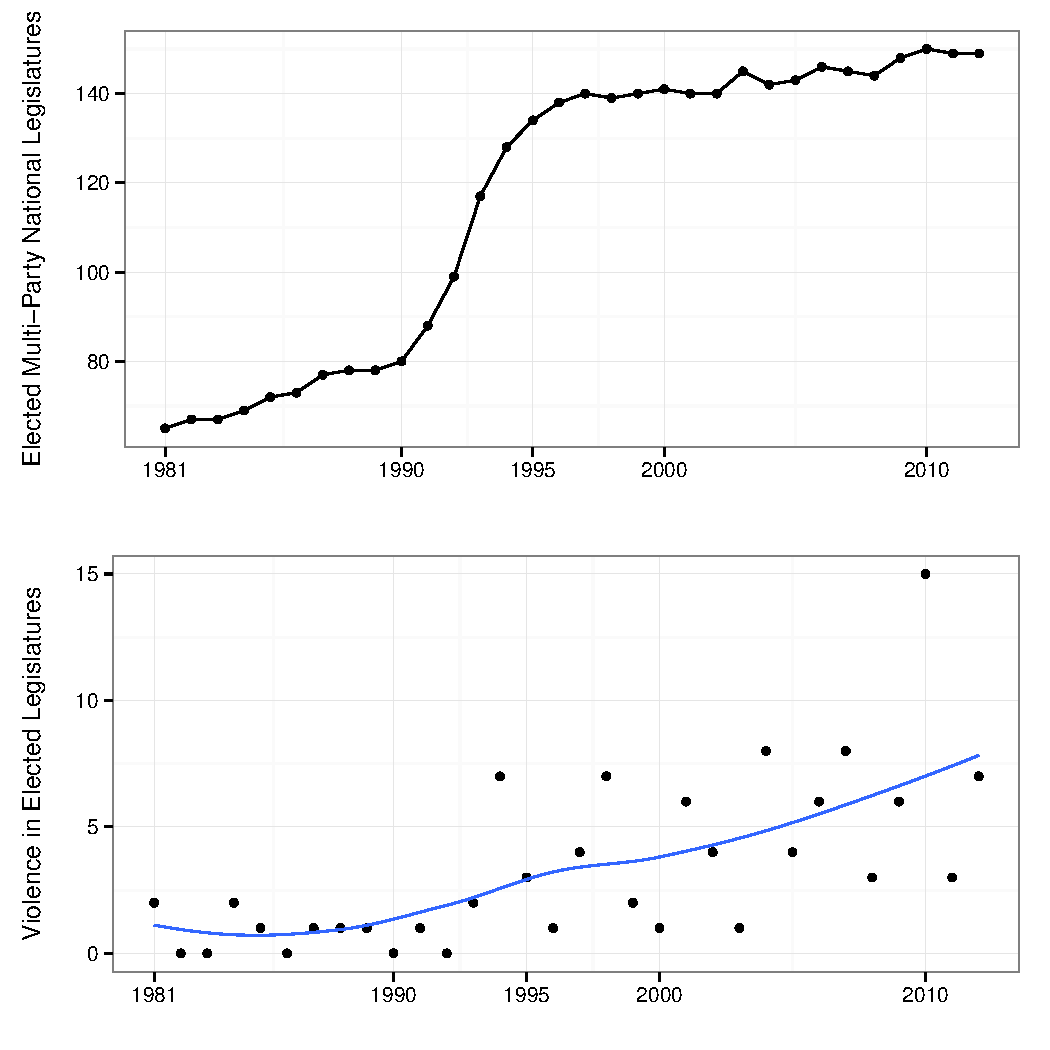
\includegraphics[width=0.8\linewidth]{figure/compareLegToViolence-1} 

\end{knitrout}
    \end{center}

    \caption{Comparing the Number of Multi-Party Elected National Legislatures to Observed Violence in These Legislatures Over Time}
    \label{elect_vs_violence}

\end{figure}


\section*{Details on Prior Correction of the Rare Logistic Regression Models}

\todo{UPDATE}

For prior correction \citep[see][]{KingRareEventsPA2001} in the models with the full sample of elected multi-party legislatures I used the observed proportion of all observations with legislative violence \change{up to 2010}{through 2012}: i.e. \change{2.1}{2.2} percent of observations up until 2010 had violence ($\tau = \frac{117}{5360} = 0.022$). There were \change{63}{109} observed incidences of violence and \change{2654}{3990} country-years from 1990 through \change{2009}{2012} in the sample, so: $\tau = \frac{109}{3390} = 0.027$.

\section*{Additional Right-hand Variables}

\todo[inline]{This section was moved from the main paper at the editor's request}

I examined a number of other legislative and societal-level variables to guard against omitted variable bias. Results from models with these variables are shown in tables \ref{outputTable.dem} and \ref{outputTable.1990_2nd}. The variables are described below. It is important to first note that overall these factors were not found to be statistically significantly associated with legislative violence nor did they substantively alter the article's core findings.

\subsubsection*{Variable Descriptions}

Gender is closely correlated with violence in society generally. Though there are many possible reasons for this that are beyond the scope of this article, women tend to commit many fewer acts of violence than men \citep[]{Schwartz2009}. Previous research has found that women's participation in parliament has an impact on government decisions to go to war \citep{Melander2005}. Perhaps if a larger proportion of legislators are women there will be less violence in the parliamentary chamber. To examine this possibility, I gathered data on the \emph{percentage of women in parliament} per country-year from two sources. Data from 1997 and after was from the Inter-Parliamentary Union \citeyearpar{IPU2013}. Data from before 1997 was from \cite{Schwartz2009}.

I included a countries' \emph{murder rate}, i.e. murders per 100,000 people, to measure a possible association between societal-level and legislative violence. The data was from \cite{UNMurder2013}, which aggregated annual murder rates from a variety of national and international sources. The data is available from 1995 through 2011.\footnote{Beyond truncating the sample somewhat, this data set unfortunately does not record Taiwan's murder rate separately from China's.}

I also included standard measures of the \emph{effective number of parliamentary parties} by votes and by seats \citep[]{Laakso1979, Taagepera1989}. The data was taken from \cite{Carey2011} before 2004 and from \cite{Gallagher2012} afterwards. Both of these measures indicate how fragmented a parliamentary party system is. Higher scores indicate that there are more parties that win either votes or seats. Neither measure produced statistically significant results, so only the results for the effective number of parties by seats are shown below.

To examine whether or not national legislative losers may be dissuaded from legislative violence because there is a possibility of gaining power at a provincial-level, I include the \emph{federalism} dummy variable from \cite{Carey2011}. I updated this from 2004 until the end of the observation period. In early models I also controlled for the government system type, i.e. if it had a presidential, parliamentary, or mixed assembly-elected presidential. This was from the DPI.

Conflict in more economically divided societies may be generally more intense. These conflicts may spill over into legislatures where they precipitate violence between members.To capture similar possible effects from economic divisions, I include {\emph{Gini coefficients of economic inequality}} from \cite{UNU2008}.\footnote{Note, for country-years with missing data I assumed that the Gini Coefficient remained constant from the last year there is data for the country, unless the span was ten years or more. If this was the case they were treated as missing.} Finally, as is common in cross-country analyses, I also include the natural logarithm (due to its right-skewed distribution) of {\emph{gross domestic product per capita}}. This data is from the World Bank's International Development Indicators \citeyearpar{WorldBank2011} and is in thousands of 2005 United States dollars.

\subsection*{Results Discussion}

\todo[inline]{Moved from main paper and changed for results with updated data.}

\paragraph{Societal-level Variables}

In general the additional societal-level variables were found to be associated with legislative violence in any of the models. Countries' murder rates were not found to be associated with violence indicating that the link between societal and legislative violence is not strong. Ethnic fractionalization was not statistically associated with legislative brawls. GDP per capita was also not found to be associated with violence. The Gini coefficient was negatively associated with brawls--more inequality was associated with less violence. This finding runs counter to expectations and requires more research to fully understand.

\paragraph{Other Political and Institutional Variables}

Results for other political and institutional variables were largely not statistically significant. The effective number of parties variables and the basic continuous government fractionalization variable was statistically significant in the analyses. Likewise, federalism did not appear to be robustly related to legislative violence across the models. All of these variables are not as directly related to legislative fairness and an ability to make credible legislative commitments at a theoretical level, compared to disproportionality, democratic age and, to a lesser extent, governing majority size. So it should not come as too much of a surprise to find that they are more loosely, if not at all, associated with legislative violence.


%%%%%%%% Elected Legislatures Results Table
\begin{table}[H]
\caption{Legislative Violence Rare Events Logistic Regression Results (Multi-Party Elected Legislature 1981-2012)}
\label{outputTable.dem}
\begin{center}
{\scalebox{0.6}{

% Table created by stargazer v.5.1 by Marek Hlavac, Harvard University. E-mail: hlavac at fas.harvard.edu
% Date and time: Wed, Mar 25, 2015 - 17:09:24
\begin{tabular}{@{\extracolsep{5pt}}lccccccccccc} 
\\[-1.8ex]\hline 
\hline \\[-1.8ex] 
 & \multicolumn{11}{c}{\textit{Dependent variable:}} \\ 
\cline{2-12} 
\\[-1.8ex] & \multicolumn{11}{c}{Violent Incident} \\ 
\\[-1.8ex] & (1) & (2) & (3) & (4) & (5) & (6) & (7) & (8) & (9) & (10) & (11)\\ 
\hline \\[-1.8ex] 
 Lower Disproportionality & $-$0.647$^{**}$ & $-$0.649$^{**}$ & $-$0.661$^{**}$ & $-$0.625$^{**}$ & $-$0.514$^{*}$ & $-$0.723$^{**}$ & $-$0.799$^{**}$ & $-$0.670$^{**}$ & $-$0.535$^{*}$ & $-$0.592$^{**}$ & $-$0.483$^{*}$ \\ 
  & (0.269) & (0.270) & (0.272) & (0.270) & (0.302) & (0.312) & (0.395) & (0.280) & (0.277) & (0.270) & (0.283) \\ 
  & & & & & & & & & & & \\ 
 Dem. Age (log) & $-$0.262$^{**}$ & $-$0.255$^{**}$ & $-$0.265$^{**}$ & $-$0.254$^{**}$ & $-$0.282$^{**}$ & $-$0.278$^{**}$ & $-$0.320$^{**}$ & $-$0.268$^{**}$ & $-$0.276$^{**}$ & $-$0.305$^{***}$ & $-$0.229$^{*}$ \\ 
  & (0.107) & (0.106) & (0.108) & (0.106) & (0.129) & (0.122) & (0.160) & (0.119) & (0.113) & (0.106) & (0.129) \\ 
  & & & & & & & & & & & \\ 
 Majority Size & $-$0.026$^{***}$ & $-$0.027$^{***}$ & $-$0.028$^{***}$ & $-$0.025$^{***}$ & $-$0.026$^{**}$ & $-$0.027$^{***}$ & $-$0.032$^{**}$ & $-$0.031$^{***}$ & $-$0.031$^{***}$ & $-$0.028$^{***}$ & $-$0.025$^{***}$ \\ 
  & (0.009) & (0.009) & (0.009) & (0.008) & (0.010) & (0.010) & (0.014) & (0.009) & (0.010) & (0.009) & (0.009) \\ 
  & & & & & & & & & & & \\ 
 Internal Armed Conflict &  & 0.676$^{**}$ & 0.647$^{**}$ & 0.658$^{**}$ & 0.635$^{*}$ & 0.819$^{**}$ & 0.430 & 0.662$^{**}$ & 0.707$^{**}$ & 0.757$^{**}$ & 0.752$^{**}$ \\ 
  &  & (0.297) & (0.297) & (0.297) & (0.342) & (0.329) & (0.501) & (0.302) & (0.302) & (0.302) & (0.310) \\ 
  & & & & & & & & & & & \\ 
 Leg. Immunity &  &  & $-$0.101 &  &  &  &  &  &  &  &  \\ 
  &  &  & (0.258) &  &  &  &  &  &  &  &  \\ 
  & & & & & & & & & & & \\ 
 Single Party Gov. &  &  & $-$0.167 &  &  &  &  &  &  &  &  \\ 
  &  &  & (0.250) &  &  &  &  &  &  &  &  \\ 
  & & & & & & & & & & & \\ 
 Political Constraints &  &  &  & $-$0.668 &  &  &  &  &  &  &  \\ 
  &  &  &  & (0.928) &  &  &  &  &  &  &  \\ 
  & & & & & & & & & & & \\ 
 Self Expression &  &  &  &  & 2.092 &  &  &  &  &  &  \\ 
  &  &  &  &  & (2.447) &  &  &  &  &  &  \\ 
  & & & & & & & & & & & \\ 
 Ethnic Frac. &  &  &  &  & $-$0.554 &  &  &  &  &  &  \\ 
  &  &  &  &  & (0.772) &  &  &  &  &  &  \\ 
  & & & & & & & & & & & \\ 
 Perc. Women in Parl. &  &  &  &  &  & 0.013 &  &  &  &  &  \\ 
  &  &  &  &  &  & (0.018) &  &  &  &  &  \\ 
  & & & & & & & & & & & \\ 
 Murder Rate &  &  &  &  &  &  & $-$0.003 &  &  &  &  \\ 
  &  &  &  &  &  &  & (0.013) &  &  &  &  \\ 
  & & & & & & & & & & & \\ 
 Federal &  &  &  &  &  &  &  & 0.178 &  &  &  \\ 
  &  &  &  &  &  &  &  & (0.347) &  &  &  \\ 
  & & & & & & & & & & & \\ 
 Gov. Frac. &  &  &  &  &  &  &  & 0.299 &  &  &  \\ 
  &  &  &  &  &  &  &  & (0.464) &  &  &  \\ 
  & & & & & & & & & & & \\ 
 No. of Parties by Seats &  &  &  &  &  &  &  &  & $-$0.081 &  &  \\ 
  &  &  &  &  &  &  &  &  & (0.093) &  &  \\ 
  & & & & & & & & & & & \\ 
 GINI &  &  &  &  &  &  &  &  &  & $-$0.038$^{**}$ &  \\ 
  &  &  &  &  &  &  &  &  &  & (0.015) &  \\ 
  & & & & & & & & & & & \\ 
 GDP per Capita (log) &  &  &  &  &  &  &  &  &  &  & $-$0.099 \\ 
  &  &  &  &  &  &  &  &  &  &  & (0.118) \\ 
  & & & & & & & & & & & \\ 
 (Intercept) & $-$0.751 & $-$0.855 & $-$0.628 & $-$0.682 & $-$3.318 & $-$0.941 & $-$0.225 & $-$0.658 & $-$0.348 & 0.776 & $-$0.295 \\ 
  & (0.535) & (0.538) & (0.633) & (0.599) & (3.057) & (0.623) & (0.804) & (0.571) & (0.732) & (0.834) & (1.001) \\ 
  & & & & & & & & & & & \\ 
\hline \\[-1.8ex] 
Observations & 1,699 & 1,699 & 1,674 & 1,674 & 909 & 1,578 & 821 & 1,563 & 1,584 & 1,677 & 1,624 \\ 
Log Likelihood & $-$279.746 & $-$277.560 & $-$276.438 & $-$276.613 & $-$203.189 & $-$225.704 & $-$138.087 & $-$258.150 & $-$263.222 & $-$272.992 & $-$247.346 \\ 
Akaike Inf. Crit. & 567.491 & 565.121 & 566.875 & 565.227 & 420.379 & 463.407 & 288.175 & 530.300 & 538.444 & 557.983 & 506.692 \\ 
\hline 
\hline \\[-1.8ex] 
\multicolumn{12}{l}{$^{*}$p$<$0.1; $^{**}$p$<$0.05; $^{***}$p$<$0.01} \\ 
\multicolumn{12}{l}{Standard errors are in parentheses. All models use robust (WEAVE) standard errors.} \\ 
\end{tabular} 

}}
\end{center}

\end{table}

%%%%%%%% Elected Legislatures Results Table from 1990--Robustness
\begin{table}[H]
\caption{Legislative Violence Regression Results (Democratic Legislature from 1990-2012)}
\label{outputTable.1990_2nd}
\begin{center}
\scalebox{0.7}{

% Table created by stargazer v.5.1 by Marek Hlavac, Harvard University. E-mail: hlavac at fas.harvard.edu
% Date and time: Wed, Mar 25, 2015 - 17:09:27
\begin{tabular}{@{\extracolsep{5pt}}lcccccc} 
\\[-1.8ex]\hline 
\hline \\[-1.8ex] 
 & \multicolumn{6}{c}{\textit{Dependent variable:}} \\ 
\cline{2-7} 
\\[-1.8ex] & \multicolumn{6}{c}{Violent Incident} \\ 
\\[-1.8ex] & (1) & (2) & (3) & (4) & (5) & (6)\\ 
\hline \\[-1.8ex] 
 Lower Disproportionality & $-$0.574$^{*}$ & $-$0.799$^{**}$ & $-$0.566$^{**}$ & $-$0.440 & $-$0.474$^{*}$ & $-$0.377 \\ 
  & (0.319) & (0.395) & (0.284) & (0.281) & (0.276) & (0.290) \\ 
  & & & & & & \\ 
 Dem. Age (log) & $-$0.306$^{**}$ & $-$0.320$^{**}$ & $-$0.291$^{**}$ & $-$0.311$^{***}$ & $-$0.322$^{***}$ & $-$0.364$^{***}$ \\ 
  & (0.131) & (0.160) & (0.128) & (0.119) & (0.111) & (0.140) \\ 
  & & & & & & \\ 
 Majority Size & $-$0.027$^{***}$ & $-$0.032$^{**}$ & $-$0.030$^{***}$ & $-$0.030$^{***}$ & $-$0.027$^{***}$ & $-$0.024$^{**}$ \\ 
  & (0.010) & (0.014) & (0.010) & (0.010) & (0.009) & (0.010) \\ 
  & & & & & & \\ 
 Internal Armed Conflict & 0.648$^{*}$ & 0.430 & 0.568$^{*}$ & 0.641$^{*}$ & 0.672$^{**}$ & 0.738$^{**}$ \\ 
  & (0.374) & (0.501) & (0.342) & (0.341) & (0.340) & (0.348) \\ 
  & & & & & & \\ 
 Perc. Women in Parliament & 0.007 &  &  &  &  &  \\ 
  & (0.019) &  &  &  &  &  \\ 
  & & & & & & \\ 
 Murder Rate &  & $-$0.003 &  &  &  &  \\ 
  &  & (0.013) &  &  &  &  \\ 
  & & & & & & \\ 
 Federal &  &  & 0.018 &  &  &  \\ 
  &  &  & (0.393) &  &  &  \\ 
  & & & & & & \\ 
 Gov. Frac. &  &  & 0.171 &  &  &  \\ 
  &  &  & (0.486) &  &  &  \\ 
  & & & & & & \\ 
 No. of Parties by Seats &  &  &  & $-$0.115 &  &  \\ 
  &  &  &  & (0.097) &  &  \\ 
  & & & & & & \\ 
 Gini &  &  &  &  & $-$0.041$^{***}$ &  \\ 
  &  &  &  &  & (0.016) &  \\ 
  & & & & & & \\ 
 GDP per Capita (log) &  &  &  &  &  & 0.073 \\ 
  &  &  &  &  &  & (0.130) \\ 
  & & & & & & \\ 
 (Intercept) & $-$0.717 & $-$0.117 & $-$0.526 & $-$0.064 & 1.004 & $-$1.319 \\ 
  & (0.650) & (0.804) & (0.594) & (0.765) & (0.854) & (1.074) \\ 
  & & & & & & \\ 
\hline \\[-1.8ex] 
Observations & 1,316 & 821 & 1,316 & 1,334 & 1,415 & 1,368 \\ 
Log Likelihood & $-$202.608 & $-$138.087 & $-$234.647 & $-$238.738 & $-$248.040 & $-$223.630 \\ 
Akaike Inf. Crit. & 417.217 & 288.175 & 483.295 & 489.475 & 508.079 & 459.260 \\ 
\hline 
\hline \\[-1.8ex] 
\multicolumn{7}{l}{$^{*}$p$<$0.1; $^{**}$p$<$0.05; $^{***}$p$<$0.01} \\ 
\multicolumn{7}{l}{Standard errors are in parentheses. All models use robust (WEAVE) standard errors.} \\ 
\end{tabular} 

}
\end{center}
\end{table}


\section*{Interactions}

\todo[inline]{Section added}

I examined a number of interactions between the article's key independent variables--lower disproportionality and democratic age--and a number of societal level and political variables. While I did not find evidence for additive relationships between most of the societal variables and legislative brawls, perhaps they mediate the effect of disproportionality or democratic age. For example, legislators in more homogenous societies might have fewer information asymmetries across partisan divides enabling them to establish credible commitments despite having a new democracy.

Tables \ref{prop_interact} and \ref{dem_interact} provide the raw estimates from these interactive models. We can see that some of the interactions contain statistically significant terms, though usually at only the 10\% level.

As in the main article, in order to evaluate the substantive significance of these findings I simulated expected probabilities for interactions that included statistically significant terms at the 10\% level and higher. I then plotted them in Figure \ref{interact_plots1} and \ref{interact_plots2}. The plots show expected probabilities for various levels of low disproportionality and democratic age at `high' and `low' values of the other variables in the interactions. Self-expression was high at 1.35 and low at 1.1. Ethnic fractionalization was high at 0.8 and low at 0.1. Gini was high at 0.6 and low at 0.2, Finally, political constraints were high at 0.7 and low at 0.1.
These fitted values are close to the variables' minimum and maximum values to enable the largest substantively meaningful contrasts.

The substantive importance of these interactions is overall very weak. Though there are some differences, the simulations illustrate that there is considerable overlap in the uncertainty surrounding most of the estimates for substantively meaningful fitted values. To the extent that the estimates are suggestive of true interactive effects, overall it appears that factors creating credible commitment problems are worsened by self-expressive values, societal divisions, and an inability to alter policy.

For example, in the top-panel of Figure \ref{prop_interact} it appears that societies where self-expressive values are more prevalent, violence is more likely when there is high disproportionality. Perhaps, legislators in these societies

The top-panel of Figure \ref{dem_interact} suggests that perhaps in new democracies violence is more likely when there is more ethnic fractionalisation. Credible commitment problems between ethnic groups could be particularly strong in these countries. The bottom-panle of Figure \ref{dem_interact} suggests that high political constraints on policy change mediate the effect of democratic age on violence. Having more and more disperse veto players make it difficult for the current majority to enact policy change, improving their ability to make credible commitments.

Again, it is important to reiterate that though these interactive effects have statistically significant terms, the substantive importance of these estimates for meaningful fitted values is very weak.



\begin{table}
    \caption{Legislative Violence Regression Results with Lower Disproportionality Interactions (Democratic Legislature from 1990-2012)}
    \label{prop_interact}
    \begin{center}
    \scalebox{0.7}{

% Table created by stargazer v.5.1 by Marek Hlavac, Harvard University. E-mail: hlavac at fas.harvard.edu
% Date and time: Wed, Mar 25, 2015 - 17:09:31
\begin{tabular}{@{\extracolsep{5pt}}lcccccc} 
\\[-1.8ex]\hline 
\hline \\[-1.8ex] 
 & \multicolumn{6}{c}{\textit{Dependent variable:}} \\ 
\cline{2-7} 
\\[-1.8ex] & \multicolumn{6}{c}{Violent Incident} \\ 
\\[-1.8ex] & (1) & (2) & (3) & (4) & (5) & (6)\\ 
\hline \\[-1.8ex] 
 Majority Size & $-$0.026$^{***}$ & $-$0.025$^{**}$ & $-$0.026$^{***}$ & $-$0.027$^{***}$ & $-$0.023$^{**}$ & $-$0.024$^{***}$ \\ 
  & (0.009) & (0.011) & (0.009) & (0.009) & (0.010) & (0.009) \\ 
  & & & & & & \\ 
 Dem. Age (log) & $-$0.216 & $-$0.304$^{**}$ & $-$0.285$^{**}$ & $-$0.327$^{***}$ & $-$0.318$^{**}$ & $-$0.287$^{**}$ \\ 
  & (0.138) & (0.134) & (0.116) & (0.114) & (0.144) & (0.113) \\ 
  & & & & & & \\ 
 Lower Disproportionality & 0.056 & 13.533$^{**}$ & $-$1.442$^{**}$ & $-$0.531 & 2.851 & $-$0.095 \\ 
  & (0.684) & (6.461) & (0.606) & (1.180) & (1.945) & (0.775) \\ 
  & & & & & & \\ 
 Lower Disp.*Dem. Age & $-$0.213 &  &  &  &  &  \\ 
  & (0.238) &  &  &  &  &  \\ 
  & & & & & & \\ 
 Self Expression &  & 6.184$^{**}$ &  &  &  &  \\ 
  &  & (3.126) &  &  &  &  \\ 
  & & & & & & \\ 
 Lower Disp.*Self Expression &  & $-$11.035$^{**}$ &  &  &  &  \\ 
  &  & (5.113) &  &  &  &  \\ 
  & & & & & & \\ 
 Ethnic Frac. &  &  & $-$0.919 &  &  &  \\ 
  &  &  & (0.746) &  &  &  \\ 
  & & & & & & \\ 
 Lower Disp.*Ethnic Frac. &  &  & 2.392$^{*}$ &  &  &  \\ 
  &  &  & (1.297) &  &  &  \\ 
  & & & & & & \\ 
 GINI &  &  &  & $-$0.038$^{*}$ &  &  \\ 
  &  &  &  & (0.020) &  &  \\ 
  & & & & & & \\ 
 Lower Disp.*GINI &  &  &  & 0.002 &  &  \\ 
  &  &  &  & (0.030) &  &  \\ 
  & & & & & & \\ 
 GDP per Capita (log) &  &  &  &  & 0.140 &  \\ 
  &  &  &  &  & (0.148) &  \\ 
  & & & & & & \\ 
 Lower Disp.*GDP Per Capita &  &  &  &  & $-$0.381 &  \\ 
  &  &  &  &  & (0.232) &  \\ 
  & & & & & & \\ 
 Political Constraints &  &  &  &  &  & $-$0.141 \\ 
  &  &  &  &  &  & (1.169) \\ 
  & & & & & & \\ 
 Lower Disp.*Pol. Constraints &  &  &  &  &  & $-$1.018 \\ 
  &  &  &  &  &  & (1.894) \\ 
  & & & & & & \\ 
 (Intercept) & $-$0.821 & $-$8.548$^{**}$ & $-$0.341 & 0.971 & $-$1.949 & $-$0.689 \\ 
  & (0.599) & (3.991) & (0.653) & (0.968) & (1.253) & (0.716) \\ 
  & & & & & & \\ 
\hline \\[-1.8ex] 
Observations & 1,437 & 808 & 1,431 & 1,415 & 1,368 & 1,413 \\ 
Log Likelihood & $-$253.938 & $-$186.618 & $-$252.307 & $-$249.650 & $-$224.022 & $-$253.219 \\ 
Akaike Inf. Crit. & 517.875 & 385.235 & 516.615 & 511.301 & 460.044 & 518.438 \\ 
\hline 
\hline \\[-1.8ex] 
\multicolumn{7}{l}{$^{*}$p$<$0.1; $^{**}$p$<$0.05; $^{***}$p$<$0.01} \\ 
\multicolumn{7}{l}{Standard errors are in parentheses. All models use robust (WEAVE) standard errors.} \\ 
\end{tabular} 

    }
    \end{center}
\end{table}

}
\begin{table}
    \caption{Legislative Violence Regression Results with Democratic Age Interactions (Democratic Legislature from 1990-2012)}
    \label{dem_interact}
    \begin{center}
    \scalebox{0.7}{

% Table created by stargazer v.5.1 by Marek Hlavac, Harvard University. E-mail: hlavac at fas.harvard.edu
% Date and time: Wed, Mar 25, 2015 - 17:09:33
\begin{tabular}{@{\extracolsep{5pt}}lccccc} 
\\[-1.8ex]\hline 
\hline \\[-1.8ex] 
 & \multicolumn{5}{c}{\textit{Dependent variable:}} \\ 
\cline{2-6} 
\\[-1.8ex] & \multicolumn{5}{c}{Violent Incident} \\ 
\\[-1.8ex] & (1) & (2) & (3) & (4) & (5)\\ 
\hline \\[-1.8ex] 
 Majority Size & $-$0.026$^{**}$ & $-$0.027$^{***}$ & $-$0.028$^{***}$ & $-$0.024$^{**}$ & $-$0.027$^{***}$ \\ 
  & (0.010) & (0.009) & (0.009) & (0.010) & (0.009) \\ 
  & & & & & \\ 
 Lower Disproportionality & $-$0.452 & $-$0.529$^{*}$ & $-$0.465$^{*}$ & $-$0.337 & $-$0.520$^{*}$ \\ 
  & (0.306) & (0.275) & (0.276) & (0.288) & (0.276) \\ 
  & & & & & \\ 
 Dem. Age (log) & $-$0.180 & 0.076 & 0.358 & 0.219 & $-$0.827$^{**}$ \\ 
  & (2.801) & (0.217) & (0.512) & (0.822) & (0.331) \\ 
  & & & & & \\ 
 Self Expression & 3.249 &  &  &  &  \\ 
  & (5.601) &  &  &  &  \\ 
  & & & & & \\ 
 Dem. Age*Self Expression & $-$0.109 &  &  &  &  \\ 
  & (2.177) &  &  &  &  \\ 
  & & & & & \\ 
 Ethnic Frac. &  & 2.375$^{*}$ &  &  &  \\ 
  &  & (1.390) &  &  &  \\ 
  & & & & & \\ 
 Dem. Age*Ethnic Frac. &  & $-$0.996$^{**}$ &  &  &  \\ 
  &  & (0.495) &  &  &  \\ 
  & & & & & \\ 
 GINI &  &  & 0.007 &  &  \\ 
  &  &  & (0.035) &  &  \\ 
  & & & & & \\ 
 Dem. Age*GINI &  &  & $-$0.019 &  &  \\ 
  &  &  & (0.013) &  &  \\ 
  & & & & & \\ 
 GDP per Capita (log) &  &  &  & 0.208 &  \\ 
  &  &  &  & (0.296) &  \\ 
  & & & & & \\ 
 Dem. Age*GDP Per Capita &  &  &  & $-$0.066 &  \\ 
  &  &  &  & (0.095) &  \\ 
  & & & & & \\ 
 Political Constraints &  &  &  &  & $-$3.944$^{*}$ \\ 
  &  &  &  &  & (2.129) \\ 
  & & & & & \\ 
 Dem. Age*Pol. Constraints &  &  &  &  & 1.436$^{*}$ \\ 
  &  &  &  &  & (0.825) \\ 
  & & & & & \\ 
 (Intercept) & $-$4.707 & $-$1.542$^{*}$ & $-$0.647 & $-$2.405 & 0.872 \\ 
  & (7.152) & (0.828) & (1.430) & (2.496) & (0.992) \\ 
  & & & & & \\ 
\hline \\[-1.8ex] 
Observations & 808 & 1,431 & 1,415 & 1,368 & 1,413 \\ 
Log Likelihood & $-$188.953 & $-$252.200 & $-$248.750 & $-$225.125 & $-$251.994 \\ 
Akaike Inf. Crit. & 389.906 & 516.401 & 509.499 & 462.251 & 515.989 \\ 
\hline 
\hline \\[-1.8ex] 
\multicolumn{6}{l}{$^{*}$p$<$0.1; $^{**}$p$<$0.05; $^{***}$p$<$0.01} \\ 
\multicolumn{6}{l}{Standard errors are in parentheses. All models use robust (WEAVE) standard errors.} \\ 
\end{tabular} 

    }
    \end{center}
\end{table}

\begin{figure}
    \begin{center}
\begin{knitrout}
\definecolor{shadecolor}{rgb}{0.969, 0.969, 0.969}\color{fgcolor}
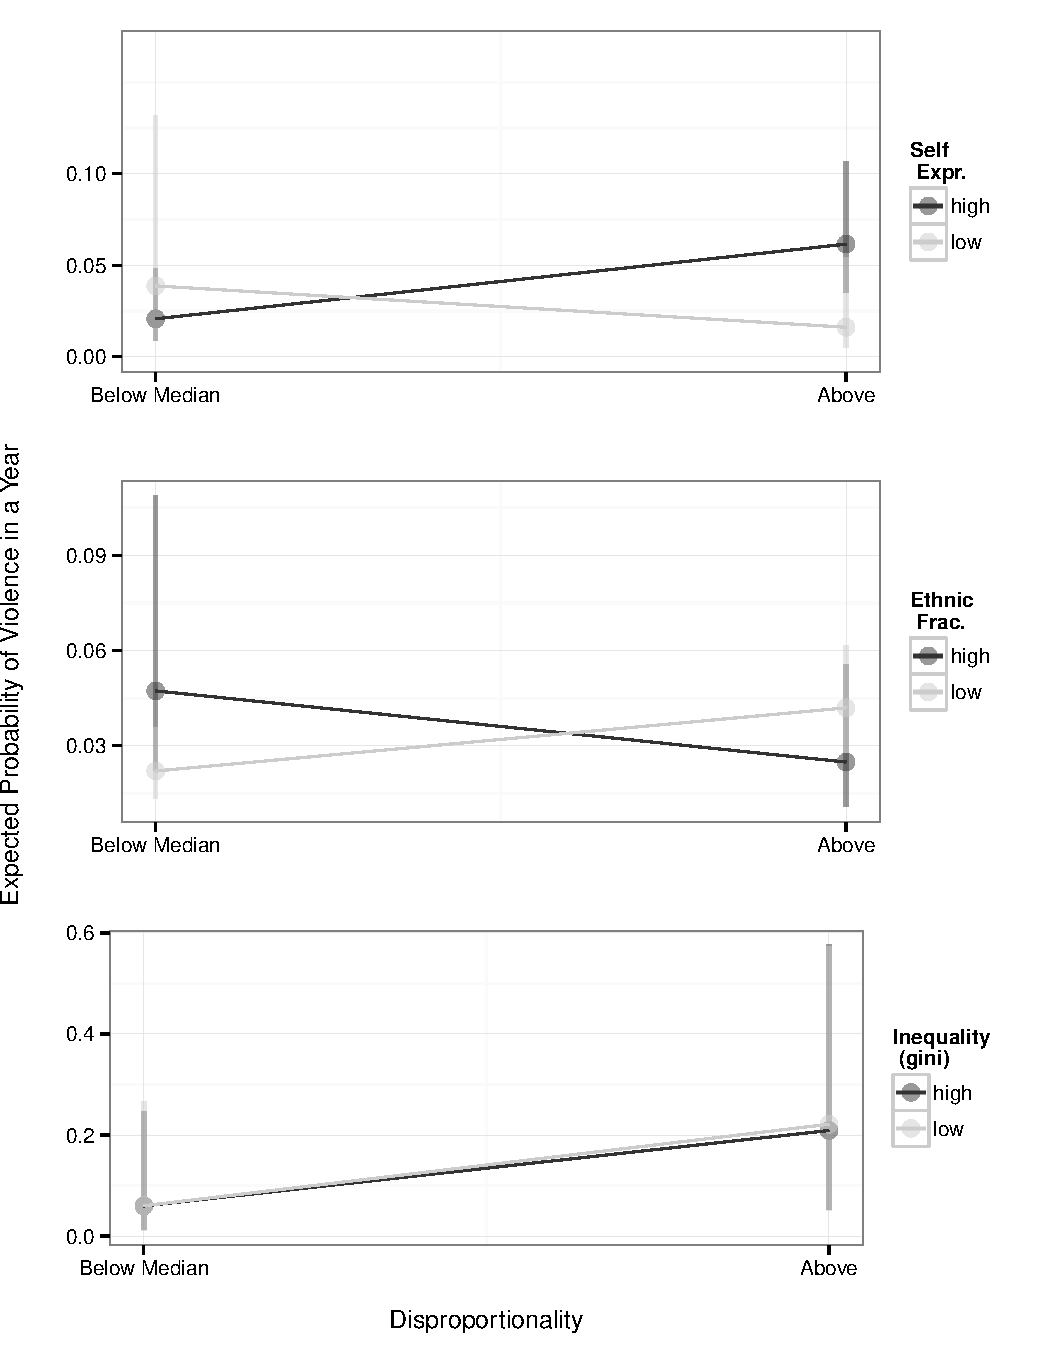
\includegraphics[width=0.95\linewidth]{figure/predProInteract-1} 

\end{knitrout}

    \end{center}
    \caption{Expected Probability of Legislative Violence in Democratic Legislatures per Year (Interactions 1)}
    \label{interact_plots1}
    \begin{singlespace}
      {\scriptsize{The graphs show the median and middle 95\% of 1000 simulations at each fitted value of the variables. The simulations use estimates from tables \ref{prop_interact} and \ref{dem_interact}. For each set of simulations all other variables were fitted at their means.}}
    \end{singlespace}
\end{figure}

\begin{figure}
    \begin{center}
\begin{knitrout}
\definecolor{shadecolor}{rgb}{0.969, 0.969, 0.969}\color{fgcolor}
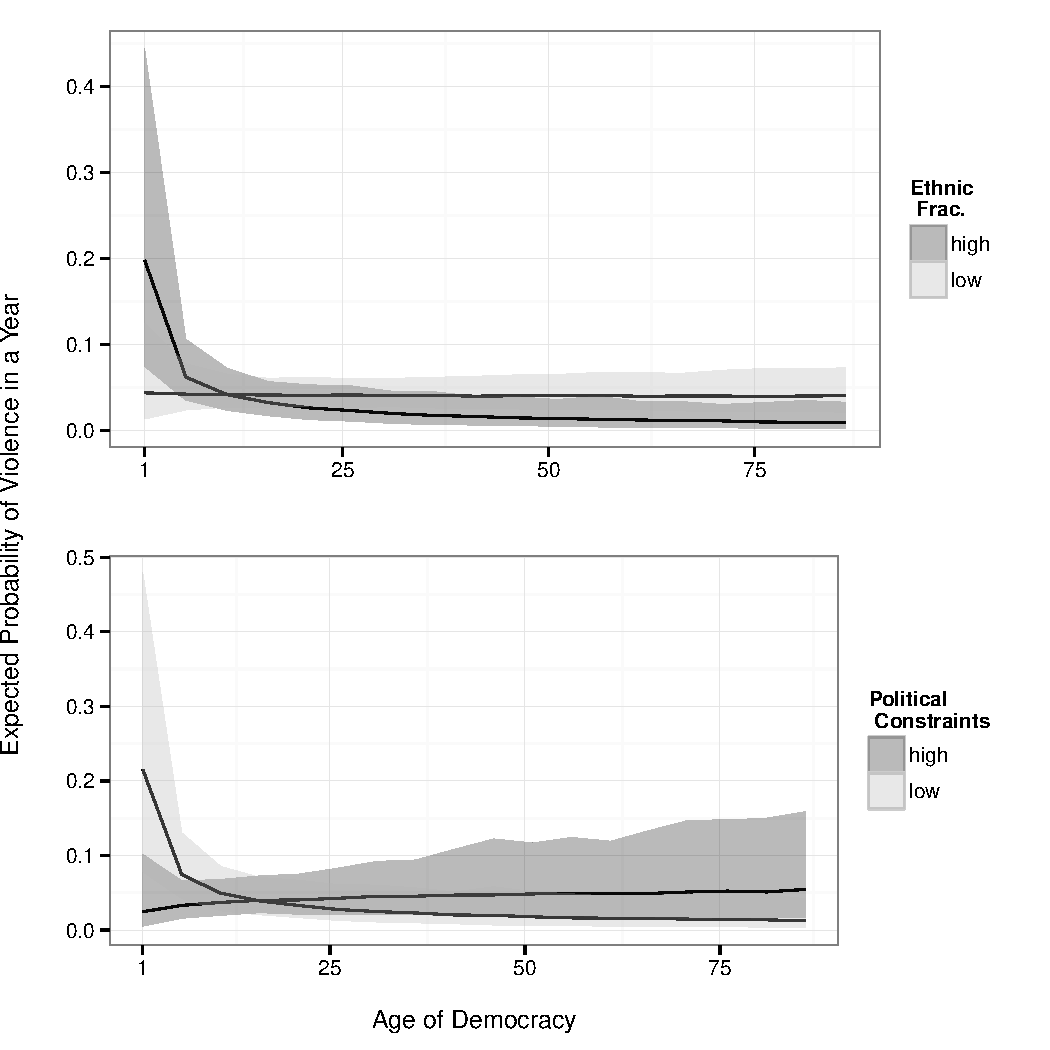
\includegraphics[width=0.95\linewidth]{figure/predProInteract2-1} 

\end{knitrout}

    \end{center}
    \caption{Expected Probability of Legislative Violence in Democratic Legislatures per Year (Interactions 2)}
    \label{interact_plots2}
    \begin{singlespace}
      {\scriptsize{The graphs show the median and middle 95\% of 1000 simulations at each fitted value of the variables. The simulations use estimates from tables \ref{prop_interact} and \ref{dem_interact}. For each set of simulations all other variables were fitted at their means.}}
    \end{singlespace}
\end{figure}


%%%%%%%%%%%%%%%%%%%%%% Figures Start %%%%%%%%%%%%%%%%%%%%%%%%%%%%%%%%%%%%%%%%%%%%%


%%%%%%%% Variable source summary table
\begin{table}[!h]
    \small
    \begin{center}
    \caption{Variable Summary}
    \label{var_summary}
    \begin{tabular}{l m{7cm} m{3.5cm}}

            \hline
            Variable & Description & Source \\
            \hline \hline
            Disproportionality & Gallagher Index of Electoral Disproportionality & \cite{Gallagher2012} \& \cite{Carey2011} \\
            ENPS & Effective number of parties by seats & \cite{Gallagher2012} \& \cite{Carey2011} \\
            ENPV & Effective number of parties by votes & \cite{Gallagher2012} \& \cite{Carey2011} \\
            Ethnic Fractionalization & Probability two randomly selected members of society are from the same ethnic group & \cite{Alesina2003} \\
            Federal & Whether a country has a federal system or not & \cite{Carey2011}, updated from 2003 by the author \\
            GDP/Capita & GDP per capita in thousands of US dollars & \cite{WorldBank2011} \\
            Gov. Fractionalization & Probability that two members of the Government will be from different parties & \cite{DPI2001} \\
            Gini & Gini Coefficient of income inequality averaged over reported sources & \cite{UNU2008} \\
            Immunity & Whether a legislators are immune from arrest and/or criminal prosecution or not & \cite{Fish2009} \\
            Internal Conflict & Internal armed conflict involving purely domestic as well as external combatants & UCDP/PRIO Armed Conflict Dataset \citep{Themner2014} \\
            LEIC & Legislative Indices of Electoral Competitiveness. Includes both the existence of a legislature and its level of electoral competitiveness. & \cite{DPI2001} \\
            Lower Disproportionality & Gallagher Index below the sample mean (6.4) & Author's calculations based on \cite{Gallagher2012} \& \cite{Carey2011}\\
            Majority & Percentage of legislature controlled by governing parties & \cite{DPI2001} \\
            Murder Rate & Murders per 100,000 population & \cite{UNMurder2013} \\
            Political Constraints & POLCONIII measure of political constraints & \cite[][updated through 2011]{Henisz2004} \\
            Polity & Polity IV Score & \cite{Marshall2009} \\
            PR & Whether a country uses a proportional representation electoral system or a plurality system & \cite{DPI2001} \\
            Self Expression & WVS self-expression indicator averaged across country-survey waves & \cite{WVS2009} \\
            System & Government system (parliamentary, presidential, or mixed & \cite{DPI2001} \\
            Trust & Average of WVS responses where 1 $=$ most people can be trusted and 2 $=$ you can't be too careful & \cite{WVS2009} \\
            Violence & Incidences of violence between legislators in the national parliamentary chamber & author \\
            Perc. Women in Parl. & Percentage of parliamentary seats held by women & \cite{WomParCrossNat} \& \cite{IPU2013} \\
            \hline

    \end{tabular}
    \end{center}
    \begin{singlespace}
        Please contact the author for detailed summary statistics. \\
        All of the data from \cite{DPI2001} was updated through 2012.
    \end{singlespace}

\end{table}

%%%%%%%%%% Correlation matrix %%%%%%%%%%
\begin{landscape}
\begin{figure}[t]

    \begin{center}

    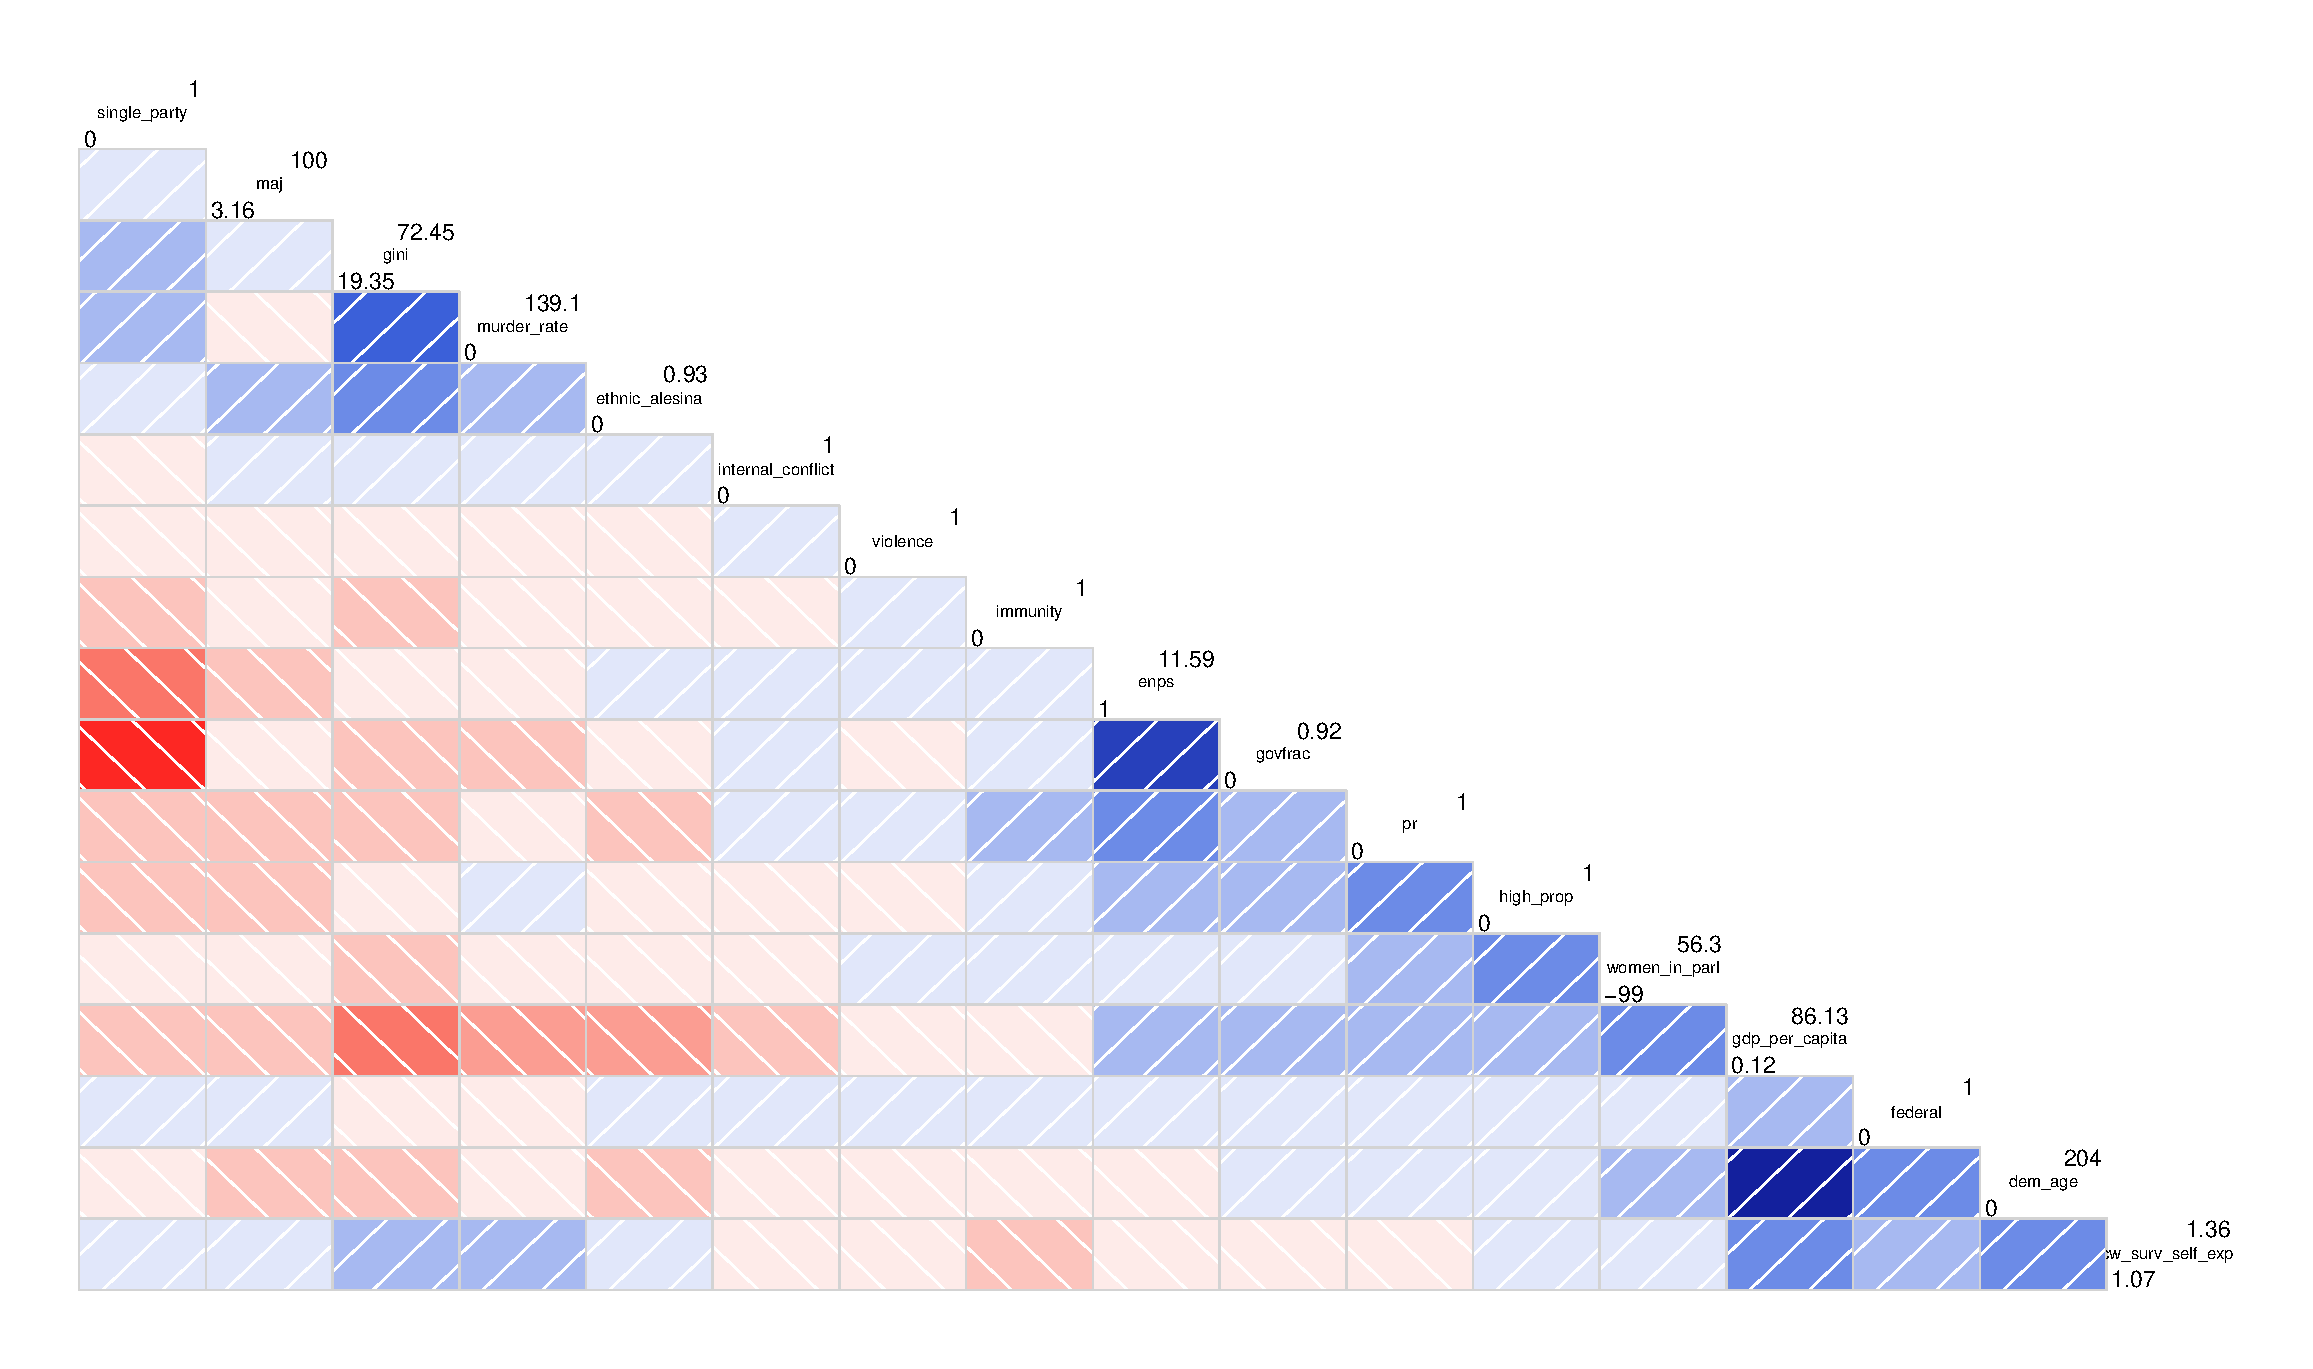
\includegraphics[scale=0.5]{corrScatter.pdf}

    \end{center}

    \caption{Correlation Matrix for Variables Included in the Analysis (Multi-Party Elected Legislatures)}
    \label{corrmatrix}

    \begin{singlespace}
        {\scriptsize{Redder squares indicate stronger negative bi-variate correlations. \\
        Bluer squares indicate stronger positive bi-variate correlations. \\
        Numbers in the diagonal squares indicate the minimum and maximum observed values of the variables in the sample.
        }}
    \end{singlespace}
\end{figure}
\end{landscape}

%%%%%%%%%%%%%%%%%%%%%% Figures End %%%%%%%%%%%%%%%%%%%%%%%%%%%%%%%%%%%%%%%%%%%%%

\bibliographystyle{apsr}
\bibliography{LegViolence}

\end{document}
